\documentclass[tikz,border=5]{standalone}

\usepackage{mathdots}

\usetikzlibrary{calc}
\usetikzlibrary{decorations.pathreplacing}
\usetikzlibrary{scopes}

\begin{document}
  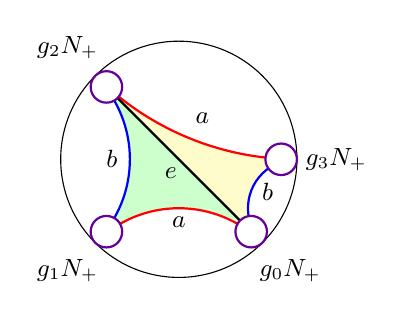
\begin{tikzpicture}
    \tikzset{font=\small}
    \begin{scope}[shift={(0,0)}]
      \draw (0,0) circle (1.5);

      \fill[thick, even odd rule, fill=yellow!20!white]
            (135:1.5) to (315:1.5)
                      arc(225: 90:0.622)
                      arc(270:225:3.615)
        ;

      \fill[thick, even odd rule, fill=green!20!white]
            (315:1.5) to (135:1.5)
                      arc(405:315:1.5        )
                      arc(135: 45:1.5        )
        ;

        \draw[thick, red ] (315:1.5) arc( 45:135:1.5);
        \draw[thick, blue] (225:1.5) arc(315:405:1.5);

        \draw[thick, red ] (  0:1.5) arc(270:225:3.615);
        \draw[thick, blue] (315:1.5) arc(225: 90:0.622);

        \draw[thick, black] (315:1.5) -- (135:1.5);

        \node at (  0:2.0) {$g_3 N_{+}$};
        \node at (135:2.0) {$g_2 N_{+}$};
        \node at (225:2.0) {$g_1 N_{+}$};
        \node at (315:2.0) {$g_0 N_{+}$};

        \draw[thick, red!40!blue, fill=white] (  0:1.5 - 0.2) circle (0.2);
        \draw[thick, red!40!blue, fill=white] (135:1.5 - 0.2) circle (0.2);
        \draw[thick, red!40!blue, fill=white] (225:1.5 - 0.2) circle (0.2);
        \draw[thick, red!40!blue, fill=white] (315:1.5 - 0.2) circle (0.2);

        \node (l01) at (270:0.80) {$a$};
        \node (l12) at (180:0.85) {$b$};
        \node (l23) at ( 60:0.60) {$a$};
        \node (l30) at (340:1.20) {$b$};
        \node (l02) at (240:0.20) {$e$};
    \end{scope}
  \end{tikzpicture}
\end{document}
